\documentclass[11pt]{article} % For LaTeX2e
\usepackage{rldmsubmit,palatino}
\usepackage{graphicx}

\title{Inverse Modular Reinforcement Learning on Human Behavior}

\author{
Shun Zhang\\
Department of Computer Science\\
University of Texas at Austin\\
Austin, TX 78712 \\
\texttt{menie482@cs.utexas.edu} \\
\And
Matthew Tong \\
Affiliation \\
Address \\
\texttt{email} \\
\And
Mary Hayhoe \\
Affiliation \\
Address \\
\texttt{email} \\
\And
Dana Ballard \\
Affiliation \\
Address \\
\texttt{email} \\
\\
}

% The \author macro works with any number of authors. There are two commands
% used to separate the names and addresses of multiple authors: \And and \AND.
%
% Using \And between authors leaves it to \LaTeX{} to determine where to break
% the lines. Using \AND forces a linebreak at that point. So, if \LaTeX{}
% puts 3 of 4 authors names on the first line, and the last on the second
% line, try using \AND instead of \And before the third author name.

\newcommand{\fix}{\marginpar{FIX}}
\newcommand{\new}{\marginpar{NEW}}

\begin{document}

\maketitle

\begin{abstract}
The \emph{title} should be a maximum of 100 characters. 

The \emph{abstract} should be a maximum of 2000 characters of text,
including spaces (no figure is allowed). You will be asked to copy
this into a text-only box; and it will appear as such in the
conference booklet. Use 11~point type, with a vertical spacing of
12~points.  The word \textbf{Abstract} must be centered, bold, and in
point size 12. Two line spaces precede the abstract.
\end{abstract}

\keywords{
enter key words here
}

\acknowledgements{We are deeply indebted to iCORE for
their generous support of RLDM2015.}  


\startmain % to start the main 1-4 pages of the submission.

\section{Introduction}

Consider the task illustrated in Figure~\ref{fig:avatar} A). The avatar is asked to
do three sub-tasks simultaneously --- 1) following the path, indicated by the gray
line on the ground, 2) getting targets, the blue cylinders, and 3) avoiding
obstacles, the pink cylinders \cite{rothkopf2013modular}.

From the reinforcement learning perspective, this task can be decomposed to be
three sub-tasks as described above.  In Figure~\ref{fig:avatar} B), if the agent
knows the distance and angle to an object, he is expected to know the optimal
action to avoid or pursue it.

A human has not done this kind of task before can achieve a good performance
easily, shown in the experiments described later. If a human knows the policies
of the sub-tasks, or sub-MDPs, he can accomplish a complicated behavior by
combining the sub-MDPs. That is,
$$Q(s, a) = \sum_i w_i Q_i (s, a)$$
where $Q_i$ is the Q value of the i-th sub-MDP, $w_i$ is the weight of the i-th
sub-MDP. $w_i \geq 0, \sum_i w_i = 1$.

% scheduling

\begin{figure}[h!]
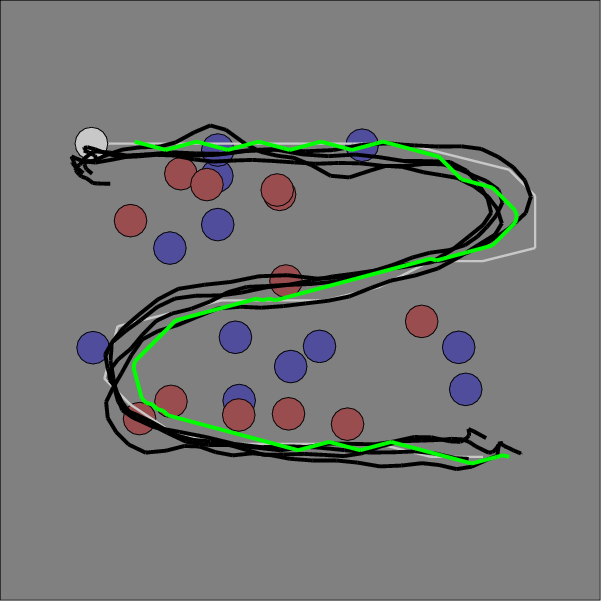
\includegraphics[width=0.5\textwidth]{task_1_room_2.png}
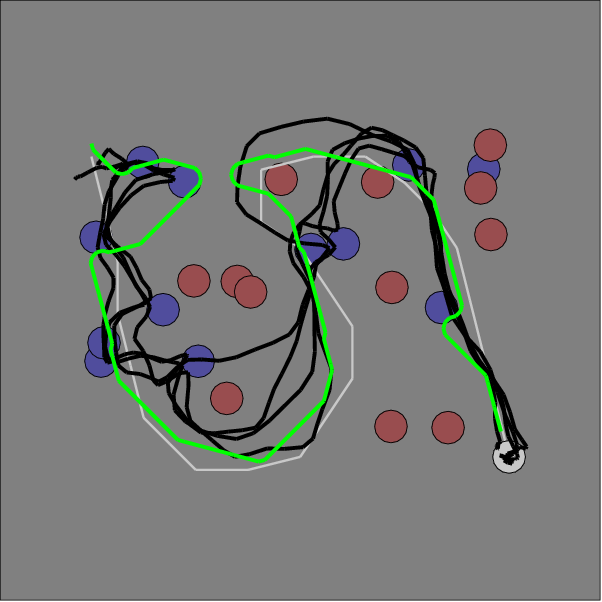
\includegraphics[width=0.5\textwidth]{task_4_room_25.png}
\caption{}
\label{fig:exp}
\end{figure}

Different weights can yield different performance. Let $w_1, w_2, w_3$ be
weights for the task of target collection, obstacle avoidance, and path
following, respectively. Let $w$ be the vector of $(w_i)_1^n$. An agent with $w
= (1, 0, 0)$ only collect targets, and one with $w = (0, 0.5, 0.5)$ may avoid
the obstacles and follow the path.

From a different perspective, can we find a weight vector to best interpret
human's behavior? In Figure~\ref{fig:exp}, there are two scenarios. Same as
Figure~\ref{fig:avatar}, the red circles are obstacles. The blue circles are
targets. The gray line is the path. The black lines are trajectories of human
data. The left figure shows the case where human follows the path and ignores
the targets and obstacles. The right figure shows the case that human does three
sub-tasks simultaneously. The human data are collected by the Center for
Perceptual Systems in University of Texas at Austin.

Now, we assume a learning agent that only knows the three sub-MDPs and the human
data. It looks at the human behavior, and finds the weights that can interpret
such behavior. Using such weights, the trajectories of our agents are drawn in
the green lines. We can tell that in the left figure, the agent puts a large
weight on path-following. In the right figure, it puts weights on all sub-MDPs.

\bibliographystyle{plain}
\bibliography{paper}

\end{document}
